\documentclass[a4paper, 14pt]{report}
\usepackage{cmap} %поиск в PDF
\usepackage[T2A]{fontenc} %кодировка
\usepackage[utf8]{inputenc} % кодировка исходного текста
\usepackage[english, russian]{babel} %локализация и переносы
\usepackage{mathtools}%для формул
\linespread{1.5}

\usepackage{graphics}
\graphicspath{{./images/}}
\usepackage{float}%"Плавающие" картинки
\usepackage{wrapfig}%Обтекание фигур (таблиц, картинок и прочего)

\usepackage{hyperref}
\usepackage{xcolor}
\definecolor{linkcolor}{HTML}{799B03}

\usepackage{algorithm}
\usepackage{algpseudocode}
\renewcommand{\listalgorithmname}{Список алгоритмов}
\floatname{algorithm}{Алгоритм}

\begin{document}
	
\begin {center} 
Минобрнауки России \\ Санкт-Петербургский политехнический университет Петра Великого \\ Институт компьютерных наук и технологий \\ Высшая школа интеллектуальных систем и суперкомпьютерных технолоий

\bigbreak
\bigbreak
\bigbreak
\bigbreak
\bigbreak
\bigbreak

\end {center}

\begin {center}
Раздаточный материал на тему: "Вербальный анализ решений
Шкала Нормализованных Упорядоченных Различий (ШНУР)"
\bigbreak
\bigbreak
\bigbreak
\bigbreak
\bigbreak
\bigbreak
\end {center}

\begin{tabular}[t]{@{}l@{\hspace{1pt}}p{.32\textwidth}@{}}
	\\
	\qquad \qquad \qquad \qquad \qquad \qquad Руководители:\\
	\qquad \qquad \qquad \qquad \qquad \qquad доцент, к.т.н. А. В. Щукин \\
	\qquad \qquad \qquad \qquad \qquad \qquad ассистент В. А. Пархоменко
\end{tabular}%

\begin{tabular}[t]{@{}l@{\hspace{1pt}}p{.56\textwidth}@{}}
	\\
	\qquad \qquad \qquad \qquad \qquad \qquad Выполнил студенты группы 3540203/90101 \\
	\qquad \qquad \qquad \qquad \qquad \qquad Зимин Юрий Геннадьевич
\end{tabular}%

\bigbreak
\bigbreak
\bigbreak
\bigbreak
\bigbreak
\bigbreak
\bigbreak
\bigbreak
\bigbreak
\bigbreak
\bigbreak
\bigbreak
\bigbreak
\bigbreak
\bigbreak
\bigbreak
\bigbreak
\bigbreak
\bigbreak


\begin {center}
Санкт-Петербург \\
2020
\end {center}

\tableofcontents
\clearpage
	
\chapter{Обзор метода вербального анализа ШНУР}

\section{Постановка задачи}

	ШНУР решает задачу выбора наилучшей альтернативы.\\
	
	$K = {K_{1},K_{2}, ..., K_{n}} $- множество критериев оценки альтернатив.\\
	
	$K =K^{\uparrow} \cup K^{\downarrow}$ , где $K^{\uparrow} $- подмножество критериев, оценку по которым нужно максимизировать,  - $K^{\downarrow}$подмножество критериев, оценку по которым нужно минимизировать. \\
	
	ЛПР – лицо, принимающее решение (эксперт осуществляющий выбор лучшего варианта по заданному алгоритму).
	
	$X_{q}={x^{k}_{q}}$ - множество оценок q-го критерия. 
	
	$A={A_{1},A_{2}, ..., A_{n}}$ – множество реальных объектов.
	
	$V=V(A_{i})$ - ценность альтернативы $A_{i}$ для ЛПР. \\
	
	Необходимо на основе предпочтений ЛПР выделить из множества А лучший объект, соответствующий наибольшему значению априорно неизвестной функции ценности $V(A_{i})$ .\\
	
	Сравнивая две альтернативы $A_{1} $и $A_{2}$ ЛПР может дать один из трех возможных ответов:
	\begin{itemize}
		\item Альтернатива $A_{1}$ предпочтительнее альтернативы  $A_{2}$ 
		\item Альтернатива  $A_{2}$  предпочтительнее альтернативы  $A_{1}$ 
		\item Альтернативы  $A_{1}$  и  $A_{2}$  одинаково предпочтительны
	\end{itemize}

	При этом не предусматривается возможность ответа «Не знаю» или «Альтернативы не сравнимы», поскольку считается, что ЛПР обладает сформулированными выше возможностям и всегда может ответить на простой вопрос.

\section{Алгоритм поиска лучшей альтернативы}

	\begin{enumerate} 
		\item Объединение близких оценок по критериям. Если оценки одинаково предпочтительны для ЛПР, их можно объединить и заменить средними значениями. 
		
		\item 	Исключение альтернатив с низкими некомпенсируемыми оценками.  Если по мнению ЛПР оценка оказалась недопустимой низкой, то вариант $A_{i}$ можно исключить из рассмотрения.
		
		\item 	Парные сравнения альтернатив. На данном шаге для каждой пары строится шкала нормализованных упорядоченных различий (рисунок~1).  Слева на шкале указывается достоинства варианта $A_{1}$ по мере убывания, а справа достоинства варианта $A_{2}$ по мере возрастания. ЛПР предлагается сравнивать достоинства начиная с предположительно больших достоинств и недостатков, т.е. двигаясь от концов шкалы по направлению к ее центру. Если одного достоинства не хватает для компенсации достоинства, то добавляется следующее достоинство с меньшим значением. 
	\end{enumerate}


	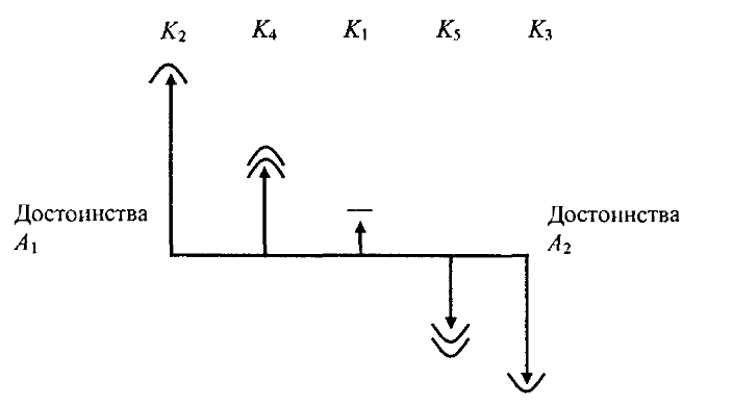
\includegraphics[scale=0.8]{1}\\
	{Рисунок~1~– Шкала Нормализованных Упорядоченных различий}\\





	Если в выборе лучшей альтернативы имеются качественные критерии, то их необходимо одинаково шкалировать:
	\begin{itemize}
		\item1 – плохая (низкая, мало);
		\item3 – средняя;
		\item5 – хорошая (высокая, много)
		\item7 – очень хорошая (высокая, много)
	\end{itemize}

	В отличии от многокритериального анализа, где выбор лучшей альтернативы без участия ЛПР, а на основе исходных оценок, результат может другим, так как какой-то критерий для ЛПР может быть необходим и иметь первостепенное значение, тогда как в многокритериальном анализе все значимость критериев одинаково.

\chapter{Программная реализация алгоритма}
	\section{Обзор реализации алгоритма}
	Система предполагает процесс авторизации/регистрации. После авторизации пользователь может создать модель (набор оценок альтернатив по каждому критерию) в следующих форматах: 
	\begin{itemize}
		\itemДемо-данные (набор готовых данных);
		\item Загрузить данные с помощью .csv файла;
	\end{itemize}

	После проверки корректности исходных данных создаются пары альтернатив и их оценки по критериям шкалируются в соответствии со шкалой нормализованных упорядоченных различий. 
	После пользователю (ЛПР) предлагается ответить на вопросы в соответствии с алгоритмом, описанным ранее. После проведение опроса ЛПР предлагается найденная лучшая альтернатива. 
	Пользователь может посмотреть раннее созданные модели и результаты по ним: лучшая альтернатива по методу ШНУР, лучшая альтернатива по мнокритериальному подходу и результаты ответов пользователя (ЛПР).
\\ \\
	\begin{tabular}{llllll}
		\hline
		Критерий                                  & Направление & A1  & A2   & A3   & A4   \\ \hline
		K1 Количество мест для парковки автомашин & max         & 400 & 300  & 250  & 150  \\
		К2: Наличие поблизости конкурентов        & min         & 1   & 5    & 3    & 5    \\
		К3 Плотность населения в радиусе 1км.     & max         & 200 & 4500 & 6000 & 7000 \\
		К4 Стоимость участка                      & min         & 6   & 16   & 12   & 20   \\
		К5 Поток общественного транспорта         & max         & 1   & 3    & 5    & 7    \\
		К6 Видимость магазина с главной улицы     & max         & 5   & 5    & 3    & 1    \\
		К7 Инфраструктура связей                  & max         & 3   & 3    & 5    & 7    \\ \hline
	\end{tabular}
Таблица 1 – Демо-данные: варианты постройки магазина\\


Средства программирования алгоритма: 
\begin{itemize}
\item Backend – Python 3.9 (Django)
\item Frontend – ReactJS
\item DB – Sqlite3
\end{itemize}

Репозиторий проекта: \href{https://github.com/ziminyuri/verbal_decision_analytics}{Github}

\section{Установка и запуск программы}
Для устновки приложения необходимо установить интерпретатор языка программирования Python (>3.7) (для работы прилоежни] на стороне сервера) и NodeJS (latest) для корректной работы ReactJs на стороне клиента.

Далее необходимо  выполнить в терминале (UNIX) следующий набор команд:
\begin{itemize}
	\item git clone ${https://github.com/ziminyuri/verbal_decision_analytics.git}$
	
	\item cd backend
	
	\item pip install -r requirements.txt
	
	\item python manage.py runserver
	
	\item cd ..
	
	\item cd frontend
	
	\item npm start
\end{itemize}

\section{Псевдокод}

	\begin{algorithm}
	\caption{Main}\label{alg:Main}
	\begin{algorithmic}[1]
		\State $M := (K, A)$
		\State $n : = len(A)$
		
		\State $k := 1$
		\For{each in n}
			\For {each b in (k, n)}
				\If a Not b
					\State $Pairs := createPairs(a, b, Pairs) $
				\EndIf
			\EndFor
		\EndFor
		
		\For {each pair in Pairs}
		\State M := Normalisation(pair. A1, pair.A2, K, M)
		\State M := Sort(M))
		\State W = FindWinner(pair.A1, pair.A2, M, K, W)
		\EndFor
	\end{algorithmic}
\end{algorithm}

\begin{algorithm}
	\caption{function Normalisation(A1, A2, K, M)}
	\begin{algorithmic}[1]
		\For {each k in K}
			\State a12 := (A1[k] + A2[k]) / 24
			\If {k.direction is max then}
				\State	a1 := A1[k]/a12
				\State a2 := A2[k]/a12
			\Else
				\State a1 := 2 - (A1[k] /a12)
				\State a2 := 2- (A2[k]/a12)
			\EndIf
			\State M.append(a1 - a2)
		\EndFor
		\State \Return M
\end{algorithmic}
\end{algorithm}

\begin{algorithm}
	\caption{function Sort(M)}
	\begin{algorithmic}[1]
		\State s := 1
		\For{each k in (length (rows) -s)}
			\For{each j in (lenght (rows) -1)}
				\If M[j]<M[j+1]
					\State temp := M[j]
					\State M[j] := M[j+1]
					\State M[j+1] := temp
				\EndIf
			\EndFor
		\EndFor
		\State \Return M
	\end{algorithmic}
\end{algorithm}


\begin{algorithm}
	\caption{function FindWinner(M)}
	\begin{algorithmic}[1]
		\State $n:=lenght (M)$
		\State $param_1, param_2 := []$
		\State $flag_1, flag_2 := True$
		\For {each i in n}
			\For{each j in n}
				\If{$flag_2$ is True}
					\State $param_1.append(K[i])$
					\State $flag_2 := False$
				\EndIf
					
				\If{$flag_1$ is True}
					\State $param_2.append(K[j])$
					\State $flag_1 := False$
				\EndIf
				
				\If {i not 0 and j not 0 and i not j}
					\State $answer := AskQuestion(param_1, param_2)$
					\If (answer is 1)
						\If $length (param_1 == 1)$
							\State win1 += 1
						\Else
							\State $param_1, param_2 := []$
						\EndIf
					\ElsIf{answer is 2}
						\If $length (param_2 == 1)$
							\State win2 += 1
						\Else
						\State $param_1, param_2 := []$
						\EndIf
					\Else
						\State $param_1, param_2 := []$
					\EndIf
				\ElsIf{i not 0}
					\State $win1 += 1$
				\ElsIf{j not 0}
					\State $win2 += 1$
					
					\algstore{bkbreak}
	\end{algorithmic}
\end{algorithm}

\begin{algorithm}
	\caption{function FindWinner(M)}
	\begin{algorithmic}[1]
		
		\algrestore{bkbreak}					
					
				\Else
					\If (win1 > win2)
						\State $winner = pair.A1$
					\Else \State $winner = pair.A2$
					\EndIf
				\EndIf
			\EndFor
		\EndFor
	\end{algorithmic}
\end{algorithm}





\chapter{Заключение}

	Метод ШНУР выбора лучшей альтернативы имеет следующие особенности:
	
	В методе используются достаточно простые процедуры выявлений предпочтений ЛПР.
	
	Диалог ведется на понятном для ЛПР языке, причем рассматриваются как качественные, так и количественные оценки альтернатив по критериям.
	
	Метод позволяет сравнить большое число альтернатив при минимальном числе вопросов к ЛПР.
	
	Метод позволяет приспособится к конкретной задаче (набору альтернатив) и выделить лучшую или предположительно лучшую альтернативу.
	
	Метод позволяет ЛПР получить объяснения сделанному выбору путем предъявления тех ответов, которые привели к полученному результату. 
	
	Во многих случаях метод помогает ЛПР в выборе лучшей альтернативы. Однако метод не всегда приводит к нужному результату, т. к. альтернативы могут быть несравнимы.

\begin{thebibliography}{3}
	\bibitem{О.И.Ларичев}
	О.И.Ларичев Вербальный анализ решений; [отв. ред. А.Б.Петровский]; Ин-т системы анализа РАН. -М.: Наука, 2006. 181 с.
\end{thebibliography}
\end{document}

\end{document}